\section{Software}
\label{sec:chapterexample}
Die Hardware ist nun vollständig und dient als Basis für die Entwicklung der Softwarekomponenten die für das System notwendig sind.
\subsection{Programmiersprachen}
Das System besteht aus mehreren Programmen und Diensten. Für die Entwicklung werden folgende Programmiersprachen eingesetzt:
\begin{itemize}
	\item Java
	\item Javascript
	\item \gls{php}
\end{itemize}
In Verbindung mit \gls{php} kommt natürlich die Markup-Languages \gls{html}5/\gls{css} zur Anwendung, welche für die graphische Darstellung der Webapplikationen notwendig ist.

\subsubsection{Java}
\label{kap:java}
Alle Dienste die serverseitig und ohne Interaktion mit dem Enduser ausgeführt werden, werden in Java programmiert. Als stark typisierte und objektorientierte Programmiersprache eignet sich Java für dieses Projekt bestens. Für Java sind auch unzählige Libraries verfügbar, insbesondere für die Hardwaresteuerung des Raspberry Pi. Eine zweite Variante wäre Python gewesen, die auch den Raspberry sehr gut unterstützt. Python ist aber zu wenig typisiert und eher für kleinere Softwarestücke gedacht.

\subsubsection{PHP/Javascript}
Sowohl die \gls{clientapp} als auch die Applikation an der \gls{aussensprechstelle} werden Web-Applikationen sein. Diese ermöglichen eine schnelle und zeitgemässe Softwareentwicklung. Für dieses Projekt ist die Systemeingriffstiefe von Webapplikationen jedenfalls ausreichend. Lediglich der Zugriff auf Mikrophon, Lautsprecher und Kamera muss garantiert werden. Ein weiterer Punkt zugunsten einer Webapplikation ist die Kompatibilität der Cross-Plattform.
\\
Aus diesem Grund haben wir uns für \gls{php} (objektorientiert) in Kombination mit Javascript/\gls{html}/\gls{css} entschieden. Eine zweite Variante wäre Java EE gewesen. Java EE eignet sich aber vor allem für grosse Softwarelösungen und bietet als gesamten Framework viel mehr als das was dieses Projekt benötigt.
\\
\subsubsection{PHP Framework: Laravel}
Für die Entwicklung der Webapplikationen wird Laravel als \gls{php} Framework eingesetzt. Laravel ist ein Open Source \gls{php} Web-Application-Framework, das sich für kleine bis zu mittelgrosse Projekte eignet. Laravel beruht auf dem ModellView-Controller-Muster und ermöglicht eine objektorientierte Programmierung in \gls{php}.

\subsection{System Übersicht}
Das System besteht aus mehreren Softwarekomponenten die zusammenarbeiten müssen (\seeref{fig:echosystem}). Die Vertraulichkeit der Kommunikation zwischen den Knoten ist dank \gls{tls} immer gewährleistet. Die einzelnen Komponenten, sowie das Thema Sicherheit, werden in den nächsten Kapiteln genauer beschrieben.

\begin{figure}[htb!]
	\begin{center}
		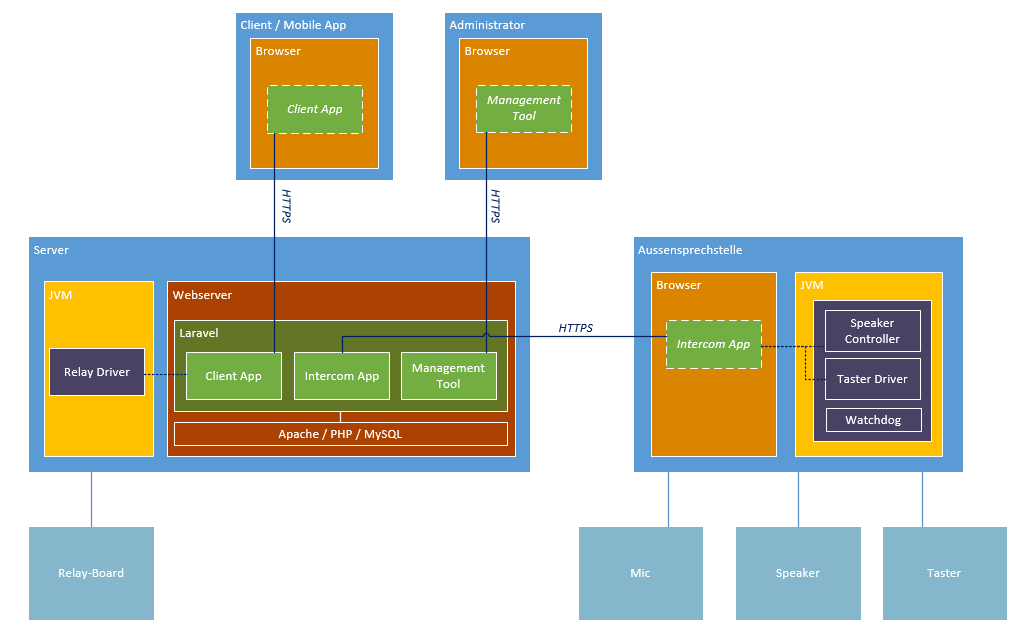
\includegraphics[width=1\textwidth]{ecosystem}
		\caption[Software Ecosystem]{Software Ecosystem}
		\label{fig:echosystem}
	\end{center}
\end{figure}

Die Software wird in zwei Gruppen unterteilt. Einerseits gibt es alle Dienste/Daemons \textit{(Violett)} die Lokal ausgeführt werden und quasi das Backend des Systems darstellen.
\\
Die zweite Gruppe beinhaltet die Webapplikationen \textit{(Grün)}, die eine \gls{gui} besitzen und für die Interaktion mit dem System gedacht sind. Darunter zählen die Client-App für die Bewohner, die Applikation bei der \gls{aussensprechstelle} wo die Bewohner angezeigt werden und das Management Tool.
\\
Die Audios/Videoskommunikation zwischen der \gls{aussensprechstelle} und den \gls{clientapp}en wird mithilfe von \gls{webrtc} realisiert. 

\subsection{Mühsame Security Policies}
Die Sicherheit spielt für dieses System eine grosse Rolle. Aus diesem Grund wurde von Anfang an geplant, den ganzen Datenverkehr mit \gls{tls} zu verschlüsseln. Auch \gls{webrtc} selber weigert sich zu funktionieren, wenn keine gültige \gls{https} Verbindung vorhanden ist.
\\
Unglücklich für die Entwicklung dieses Prototyps sind die immer mühsamere Security-Policies der heutigen Browser. Es ist zum Beispiel nicht mehr möglich, den Browser so einzustellen, dass die Zertifikatfehler ignoriert werden. Das hat als Folge, dass auch während der Entwicklung das Zertifikat gültig und signiert sein muss, ansonsten funktioniert \gls{webrtc} nicht.
\\
Dies hat uns während der Entwicklung sehr viel Zeit gekostet. Zertifikate sind immer an einem Hostname oder an einer \gls{ip} Adresse gebunden. Folge dessen mussten wir bei jeder Netzwerkanpassung alle Zertifikate nochmals generieren.
\\
Zusätzlich hat Google Chrome während der Entwicklung dieses Projekts mit der
Version 58 die Security Policies geändert. Nach dem Update brauchten die SelfSigned-Certificates ein zusätzliches Feld für den Subject-Alternative-Name (SAN). Im Netz war am Anfang sehr wenig Hilfe zu finden und das hat auch nochmals viel Zeit gekostet.


\begin{quote}
	\textit{
		"[...] RFC 2818 describes two methods to match a domain name against a certificate: using the available names within the subjectAlternativeName extension, or, in the absence of a SAN extension, falling back to the commonName. The fallback to the commonName was deprecated in RFC 2818, but support remains in a number of TLS clients, often incorrectly. [...]"
	} 
	\\
	\nocite{} [ Deprecations and Removals in Chrome 58, developers.google.com ]
\end{quote}

\subsection{WebRTC}
\label{kap:webrtc}
\gls{webrtc} ist ein offener Standard, der eine Sammlung von Kommunikationsprotokollen und API beinhaltet. Die Standardisierung wird mehrheitlich betrieben und von Google, Mozilla Foundation und Opera Software unterstützt. \gls{webrtc} basiert auf \gls{html}5 und Javascript und die Audio/Video Übertragung erfolgt über eine direkte Verbindung zwischen den Sprechpartnern (Peer-to-Peer).
\\
\\
\gls{webrtc} wird hauptsächlich für die Entwicklung von Videokonferenzprogrammen verwendet. Die Natur dieses Projekt ist allerdings nicht dieselbe wie die herkömmliche Real-Time-Communication Applikationen. Glücklicherweise wurde \gls{webrtc} so entwickelt, um möglichst viel Flexibilität zu garantieren. Aus diesem Grund beinhaltet der \gls{webrtc}-Standard keine Definition für den SignalingProcess, welcher zusammen mit dem \textbf{ICE} (Interactive Connectivity Establishment) für den Verbindungsaufbau zwischen den Sprechpartnern zuständig ist.

\begin{quote}
	\textit{
		"The thinking behind \gls{webrtc} call setup has been to fully specify and control the media plane, but to leave the signaling plane up to the application as much as possible. The rationale is that different applications may prefer to use different protocols, such as the existing SIP or Jingle call signaling protocols, or something custom to the particular application, perhaps for a novel use case. [...]"
	} 
	\\
	\nocite{} [ Sam Dutton, HTML5Rocks.com ]
\end{quote}

\subsubsection{Signaling Process}
\label{kap:signaling}
Ähnlich wie bei \gls{voip}-Telefonie \textit{(\gls{sip})}, brauchen die Sprechpartner, um die Verbindung zu initialisieren, einen gemeinsam bekannten Knoten (\seeref{fig:signaling}). In den meisten Fällen ist einem Partner die logische Adressierung des anderen Partners nicht bekannt. Es besteht also keine Möglichkeit um eine \gls{p2p} Verbindung auf einmal zu starten.

\begin{figure}[htb!]
	\begin{center}
		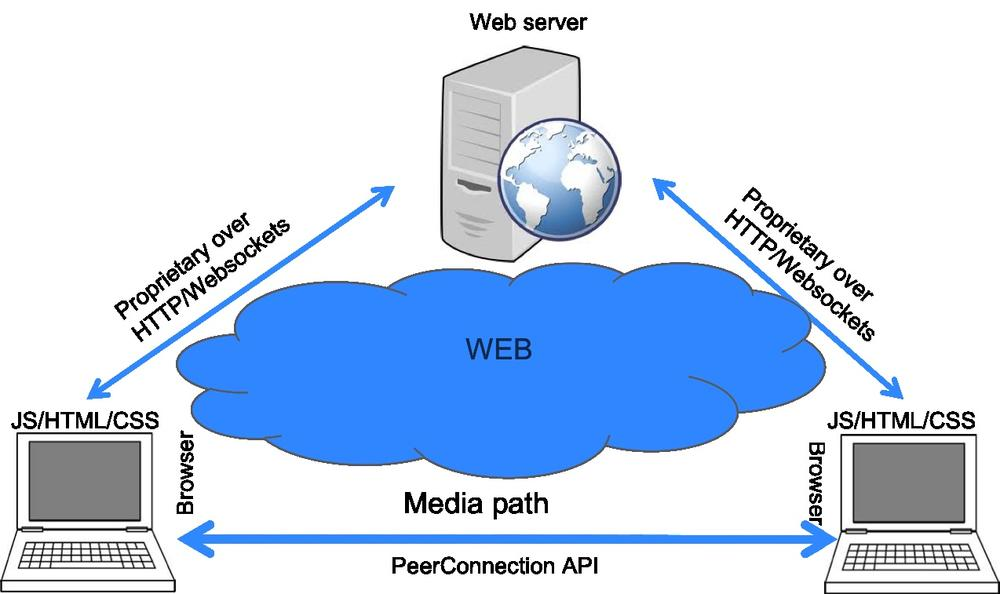
\includegraphics[width=0.75\textwidth]{signalingprocess}
		\caption[Der Signaling Prozess]{Der Signaling Prozess}
		\label{fig:signaling}
	\end{center}
\end{figure}

Im unseren Fall wäre dies theoretisch möglich, da die Position der \gls{aussensprechstelle} bzw. des Servers immer dieselbe sind. Allerdings wurde \gls{webrtc} nicht so konzipiert. Die Standard \gls{webrtc} \gls{api} beinhaltet kein Konstrukt um eine Verbindung anhand von bekannten \gls{ip}-Adressen aufbauen zu können.
\\
Im Internet sind es mehrere Signaling-Server-Libraries verfügbar, diese sind allerdings für andere Anwendungen gedacht. Im unseren System wird beispielsweise nie ein Anruf von der \gls{aussensprechstelle} zur \gls{clientapp} gestartet, sondern lediglich umgekehrt.
\\
Für die Absichten unseres Projekts wurde ein eigener Signaling-Server entwickelt, der auf dem Server ausgeführt wird. Somit bleibt der Datenverkehr zwischen der \gls{clientapp} und der\gls{aussensprechstelle} während des ganzen Ablaufes innerhalb des lokalen Netzwerkes. Das aber natürlich nur, solange der Bewohner sich zu Hause befindet.

\subsubsection{STUN Servers \& Remote Verbindung}
\label{test}
Eine Anforderung des Systems ist die Möglichkeit, auch ausserhalb des Heimnetzes mit den \gls{aussensprechstelle} sich verbinden zu können. Hier stellt das \gls{nat}-Protokoll (Network Adress Translation) ein Problem dar.

Eine Anforderung des Systems ist die Möglichkeit, auch ausserhalb des Heimnetzes, sich mit der \gls{aussensprechstelle} verbinden zu können. Hier stellt das \gls{nat} Protokoll ein Problem dar.
\\
Nach dem Signaling-Prozess wird das \gls{ice}-Prozess gestartet. Hier tauschen sich die zwei Partner Informationen über die eigene Adressierung und den \textit{best path} aus. Falls sich ein Sprechpartner hinter einem \gls{nat}-Knoten befindet, wird für den anderen unmöglich sein eine Verbindung aufzubauen. Hier kommen die \gls{stun}-Server im Spiel. 
Ähnlich wie beim Signalisierungsprozess stehen \gls{stun}-Server als Hilfe für den Verbindungsaufbau da (\seeref{fig:stun}).

\begin{figure}[htb!]
	\begin{center}
		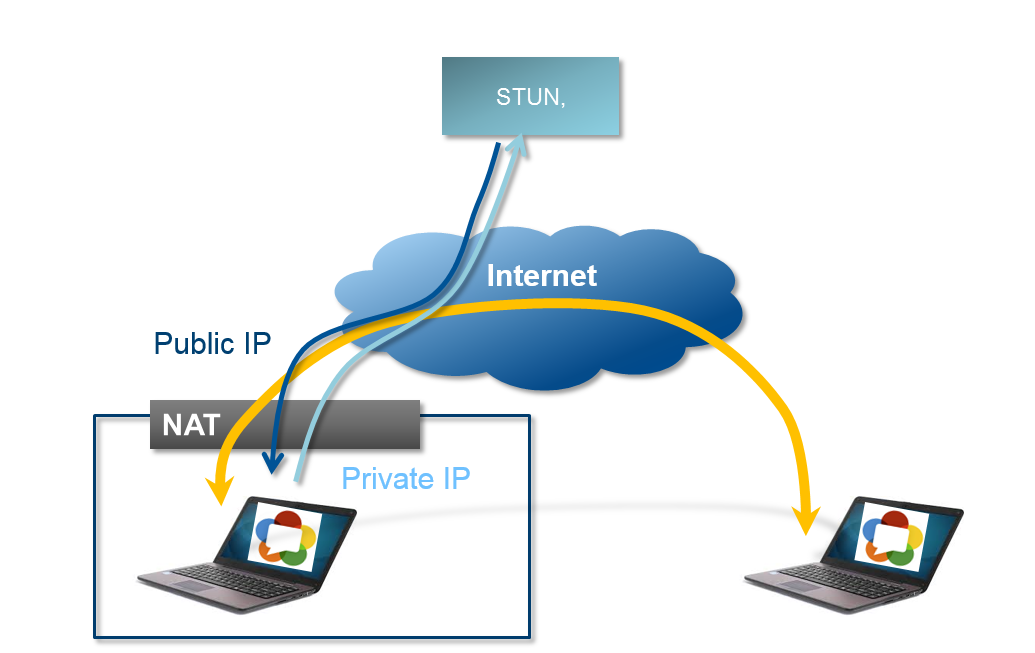
\includegraphics[width=0.75\textwidth]{stun}
		\caption[STUN Server]{STUN Server}
		\label{fig:stun}
	\end{center}
\end{figure}

\gls{stun}-Server informieren die Clients über jegliche \gls{nat} Konfigurationen die sich dazwischen befinden würden. Die beide Sprechpartner erhalten somit Informationen über welche Ports und öffentliche Adressen die Verbindung initialisiert werden kann. Für die Entwicklung dieses Projektes werden die Google-\gls{stun}-Server verwendet, welche kostenfrei zur Verfügung stehen.
\\
Falls sich beide Sprechpartner im gleichen lokales Netzwerk befinden, werden keine \gls{stun}-Server benötigt und der gesamte Datenverkehr bleibt innerhalb des Heimnetzwerkes.

\subsection{Webapplikationen}
\label{kap:webapp}
Während die verschiedene Java Dienste relativ kleine Programme sind, besteht den gesamten Quellcode der Webapplikationen aus mehreren tausende Codezeilen. 
\\
Das \gls{php}-Backend im Zusammenarbeit mit Javascript auf der Clientseite ist für die meisten Aufgaben der Anlage sowohl auch für einen Teil der Sicherheitsaspekte zuständig.

\subsubsection{Client Webapplikation}
Der Bewohner muss über eine Applikation verfügen, die auf dem Tablet oder Handy ausführbar sein muss. Mithilfe dieser App muss der Enduser folgendes können: Sich mit allen \gls{aussensprechstelle}n verbinden können, ein Videosignal von der Kamera aller Eingänge erhalten, alle Türe öffnen und mit der Person bei der Türe über die Anlage kommunizieren können.
\\
\begin{figure}[htb!]
	\begin{center}
		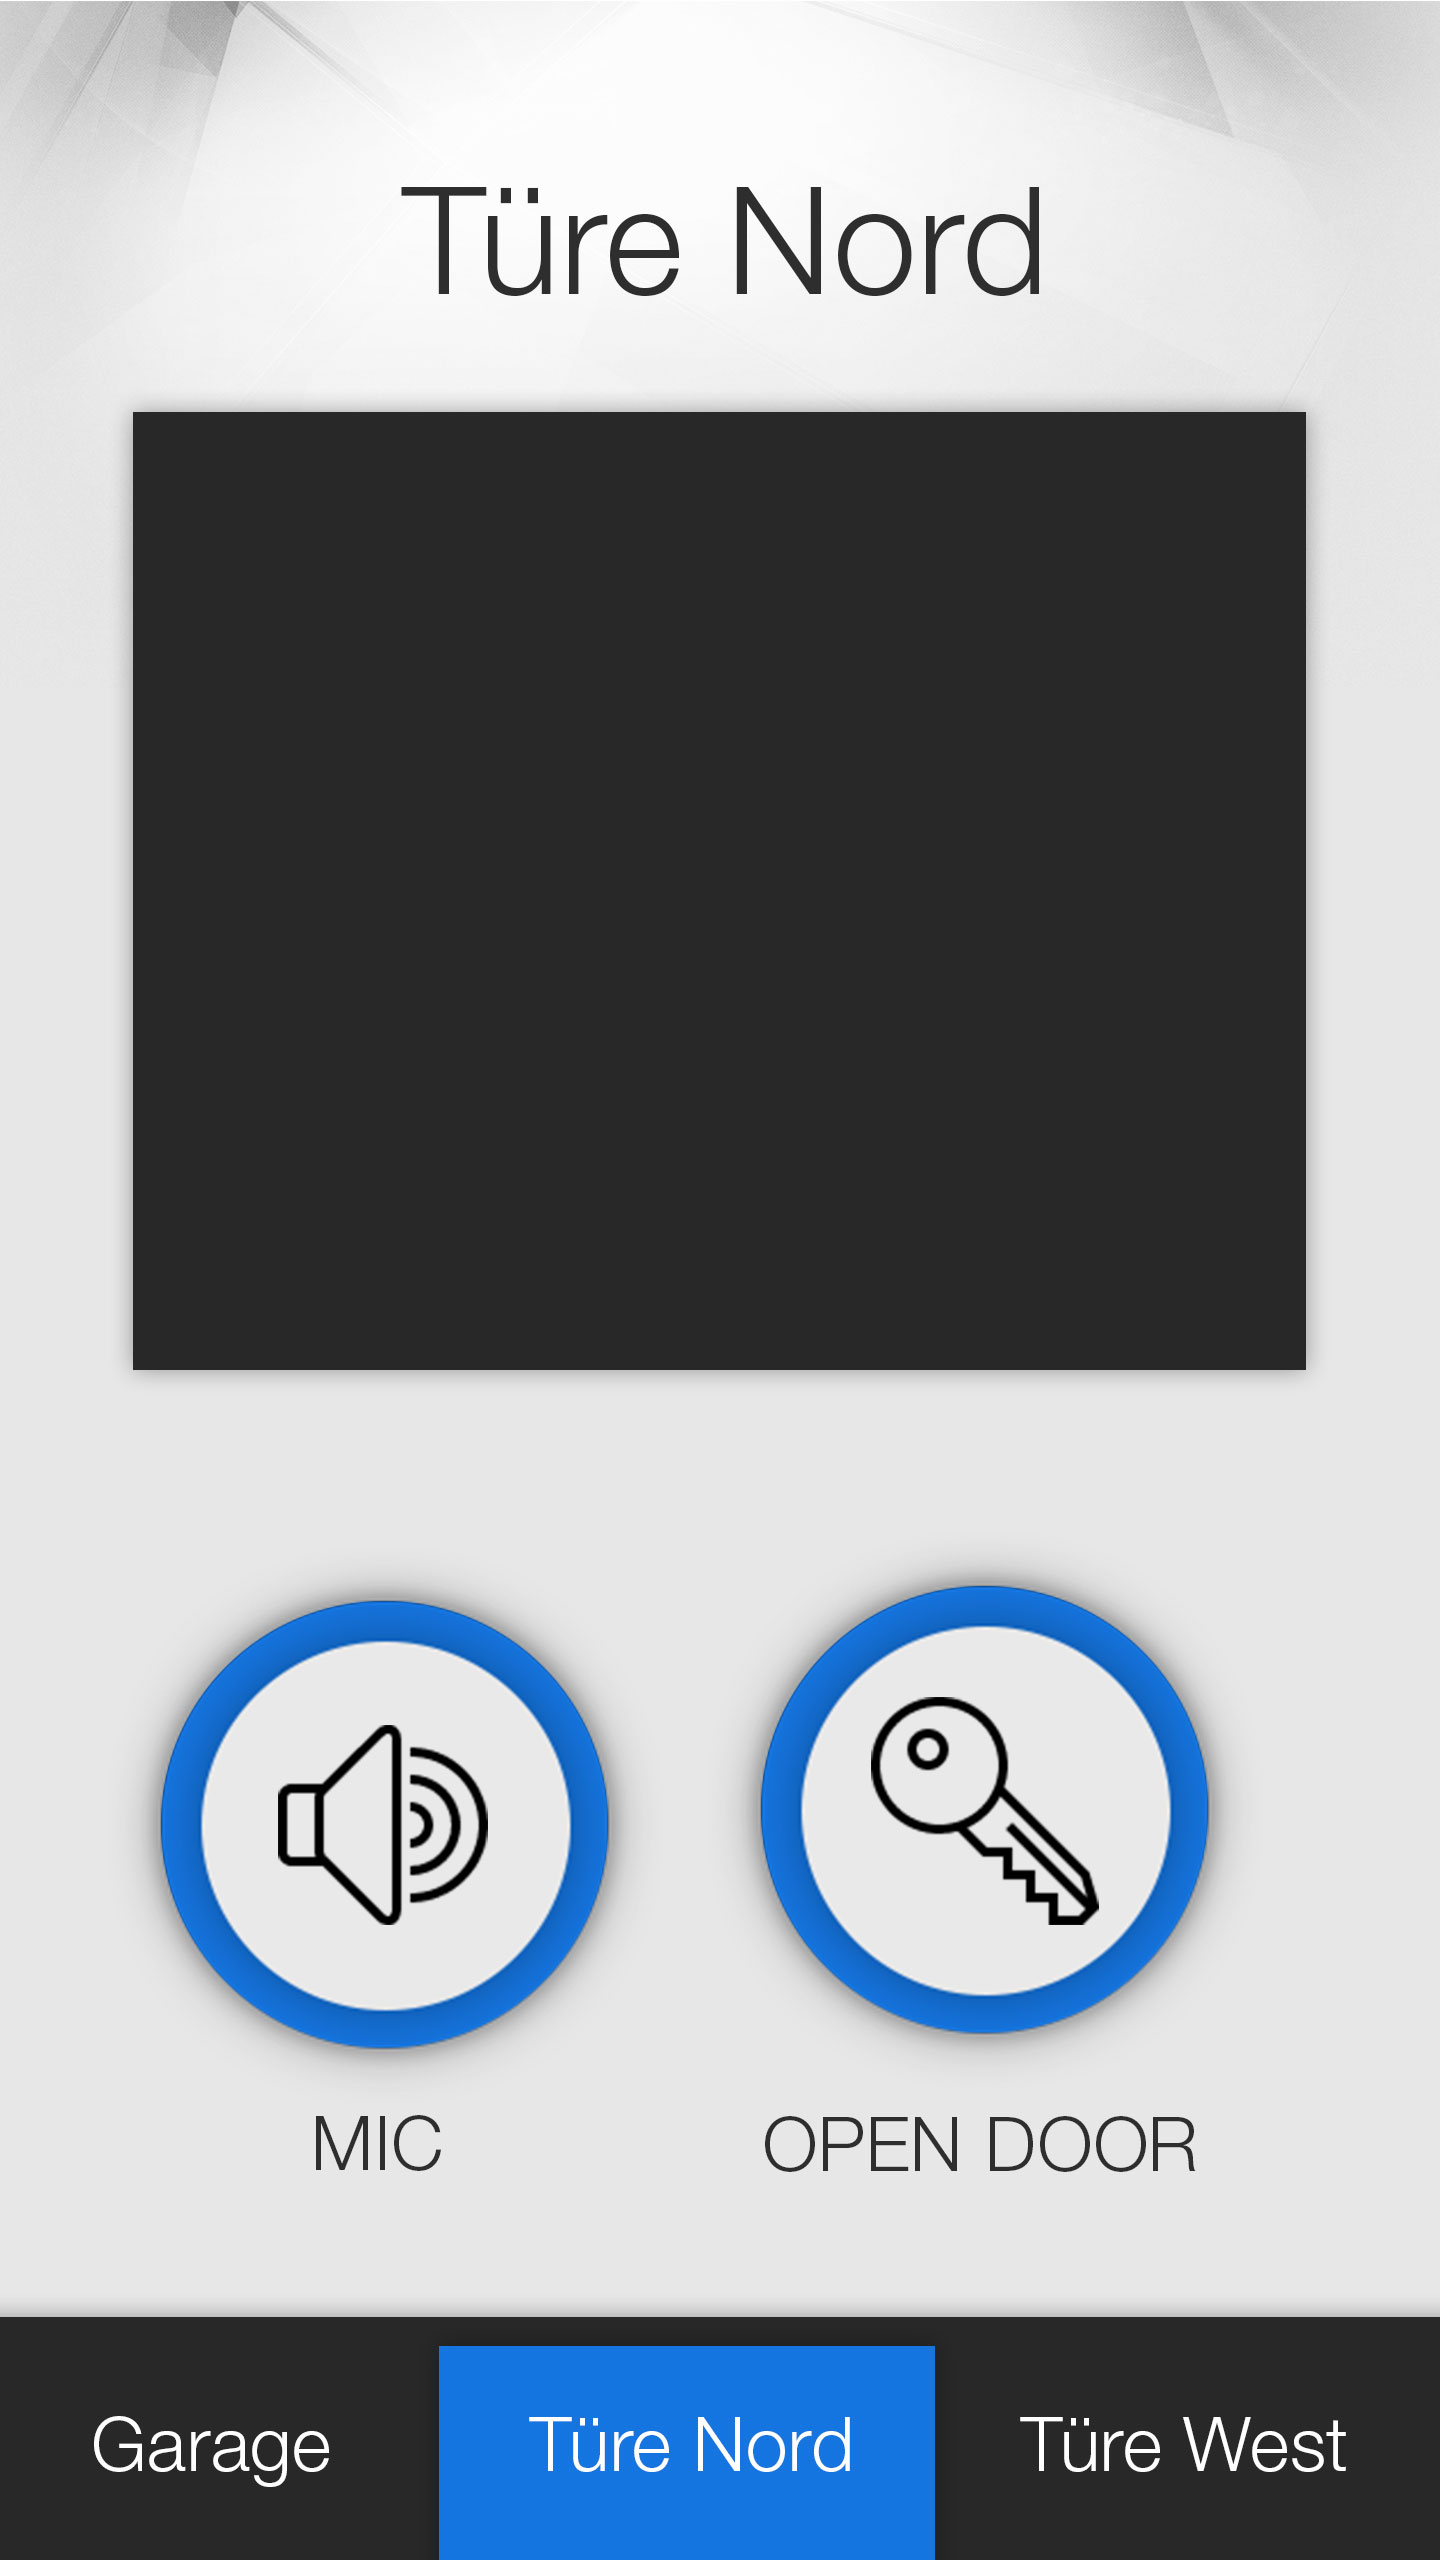
\includegraphics[width=0.35\textwidth]{clientDemo}
		\caption[Design der Client-Webapp]{Design der Client-Webapp}
		\label{fig:clientDemo}
	\end{center}
\end{figure}
\\
Die \cref{fig:clientDemo} zeigt das Design der Webapplikation, hier speziell die Smartphone Version. Dank einem Responsive-Design wird die selbe Applikation auch auf andere Geräte wie z.B. Tablets oder Computers passend angezeigt.
\\ 
Beim Design-Entwurf standen Übersichtlichkeit und Benutzerfreundlichkeit im Vordergrund. Aus diesem Grund werden die Tasten für die Audio-Kommunikation und für die Öffnung der Türe gross Angezeigt. Das Videostream der ausgewählten Türe wird sofort angezeigt und benötigt keine weitere Interaktion.
\\
\\
\textbf{Notifications}
\\
Wenn jemanden bei der Türe klingelt, wird eine Notification angezeigt. Um das zu erfolgen, muss die Webapplikation mindestens einmal gestartet werden. Dank den Notifications können auch Verpasste besuche an einem Späteren Zeitpunkt gesehen werden. 


\subsubsection{Aussensprechstelle Webapplikation}
\label{sec:AussensprechstelleWebapplikation}
Die \gls{aussensprechstelle} ist mit einem Bildschirm ausgestattet, der die Bewohnerliste anzeigt. Mithilfe von drei Schaltern kann man durchblättern und die Bewohner können angerufen werden (\seeref{fig:doordesign}).
\\
\\
Währen der Bewohner die Möglichkeit hat, die Person an der Türe zu sehen, erhaltet der Besucher an der Türe kein Videosignal, auch wenn dies technisch absolut möglich wäre. Als Bewohner will man aber die Möglichkeit haben die Türe nicht zu öffnen oder dem Besucher die eigene Präsenz gar nicht bekannt zu geben.

\begin{figure}[htb!]
	\begin{center}
		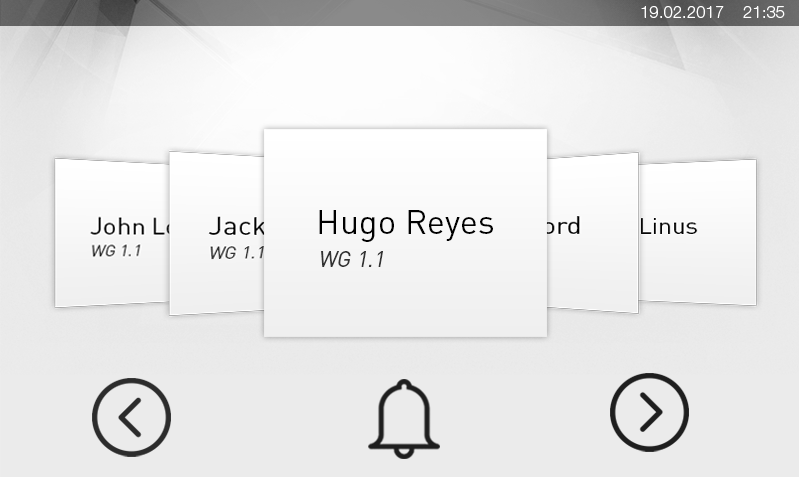
\includegraphics[width=0.70\textwidth]{doordesignbeta}
		\caption[Design der Client-Webapp]{Design der Aussensprechstelle-Webapp}
		\label{fig:doordesign}
	\end{center}
\end{figure}


\textbf{Probleme bei der Videoübertragung}
\\
Nach dem ersten Test der Webapplikationen ist ein weiteres Problem aufgetaucht. Die Qualität der Videoübertragung war nicht immer befriedigend. Das Problem ist aber erst aufgetaucht, nach dem Deploy der Webapplikationen auf die endgültige Hardware installiert wurde.
\\
Nach eine Problemanalyse konnte man folgendes feststellen:
\\
\\
Für das Video-Encoding verwendet \gls{webrtc} das VP8 Codec, da die Codierung im Gegensatz zur Decodierung, wie bei der Mehrheit solcher Systeme, sehr leistungsintensiv ist. Die \gls{aussensprechstelle} muss im Stande sein, die Codierung in Real-Time auszuführen, was den Raspberry Pi an seinen Grenzen bringt. Obwohl eine Kamera mit hoher Auflösung im Einsatz ist, wird \gls{webrtc} im Folge des niedrigen Framerates die Qualität des Stream verringern. Sobald die Qualität herabgesetzt ist, ist der Raspberry wieder im Stand die Codierung in Echtzeit durchzuführen. 
\\
Aufgrund der hohen Überlastung des Prozessors während der Kodierung, tauchen zusätzlich Wärmeabfuhrprobleme auf. Eine verlängerte Videostreaming-Session mit erhöhten Umgebungstemperaturen, könnte den Raspberry zum Absturz bringen.
\\
Der Raspberry Pi 3 war während der Entwicklungsphase des Prototyps die richtige Entscheidung. Hauptgrund waren die hohe Kompatibilität, die Standardisierung eines sehr gut etablierten Produktes und die Stabilität. Dazu kommen noch die unzähligen Infos, Dokumentationen die im Internet über diese Micro Controller zu finden sind.
\\
\\
\textbf{Alternative}
\\ 
Mit den gesammelten Erfahrungen während der Prototypentwicklung könnte eine bessere Alternative zur Raspberry für eine Weiterentwicklung der Anlage ausgewertet werden.
\\
Der Microcontroller Banana Pi M3 bietet im Gegensatz zum Raspberry erheblich mehr Datenverarbeitungsleistung (\seeref{tbl:microcontrollerComparison})). Dazu unterstützen diese Microcontroller die \gls{h264} Hardwareacceleration und der Videostream kann somit weiterhin optimiert werden.

\begin{table}[]     
	\centering
	\label{microcontrollerComparison}
	\begin{tabular}{l|ll}
		\multicolumn{1}{r|}{} & Raspberry Pi Model 3 & Banana Pi M3 \\ \hline
		CPU Cores             & 4                    & 8            \\ \hline
		CPU Design            & Cortex A53           & Cortex A7    \\ \hline
		CPU Frequenz          & 1.2GHz               & 1.8GHz       \\ \hline
		Memory                & 1GB DDR2             & 2GB DDR3     \\ \hline
		Memory Frequenz       & 400MHz               & 672MHz       \\ \hline
		H264 Decoding         & 1080P30              & 1080P60      \\ \hline
		H264 Encoding         & 1080P30              & 1080P60      \\ \hline
		Preis				  & CHF 50.0             & CHF 99.00    \\ \hline
	\end{tabular}
	\caption{Verwendete Raspberry Pi im Vergleich mit Banana Pi  als Alternative}
	\label{tbl:microcontrollerComparison}
\end{table}
Ein weiterer Vorteil des Banana Pi ist, dass der Raspbian \gls{os} ebenfalls unterstützt wird. Das mit dem Projekt mitgelieferte Image des Betriebssystems für die \gls{aussensprechstelle}n könnte somit auf den neuen Microcontroller mit geringerem Aufwand aufgespielt werden. Auch die Verkabelung sollte  kein Problem darstellen, da die Pinbelegung eins zu eins die des Raspberrys entspricht.
\\
\subsubsection{Management Tool}
\label{kap:managementtool}
Um eine schnellere Inbetriebnahme und eine zentrale Verwaltung des Systems zu gewährleisten, wurde das \gls{managementtool} entwickelt. Diese Webapplikation, die die Erfassung von \gls{aussensprechstelle}n und Bewohnern ermöglicht, wurde mit Webtechnologien entwickelt (\gls{html}, \gls{php}, Javascript) und wird zusammen mit den \gls{mysql}-Datenbank auf dem lokalen Raspberry-Server gehostet. Aus Sicherheitsgründen werden alle eingehenden und ausgehenden Verbindungen mittels\gls{tls} abhörsicher aufgebaut.
\\
Grund für das Einsetzten von Webtechnologien sind die Plattformunabhängigkeit sowie die Einfachheit und die Standardisierung der Sprachen. Beim ersten Prototyp lag der Fokus auf die funktionalen Eigenschaften des Tools. Bei einer zukünftigen Weiterentwicklung des Produkts kann man, dank der Webtechnologien, mit geringerem Aufwand das Tool skalieren bzw. neue Features hinzufügen.
\\

\begin{figure}[htb!]
	\begin{center}
		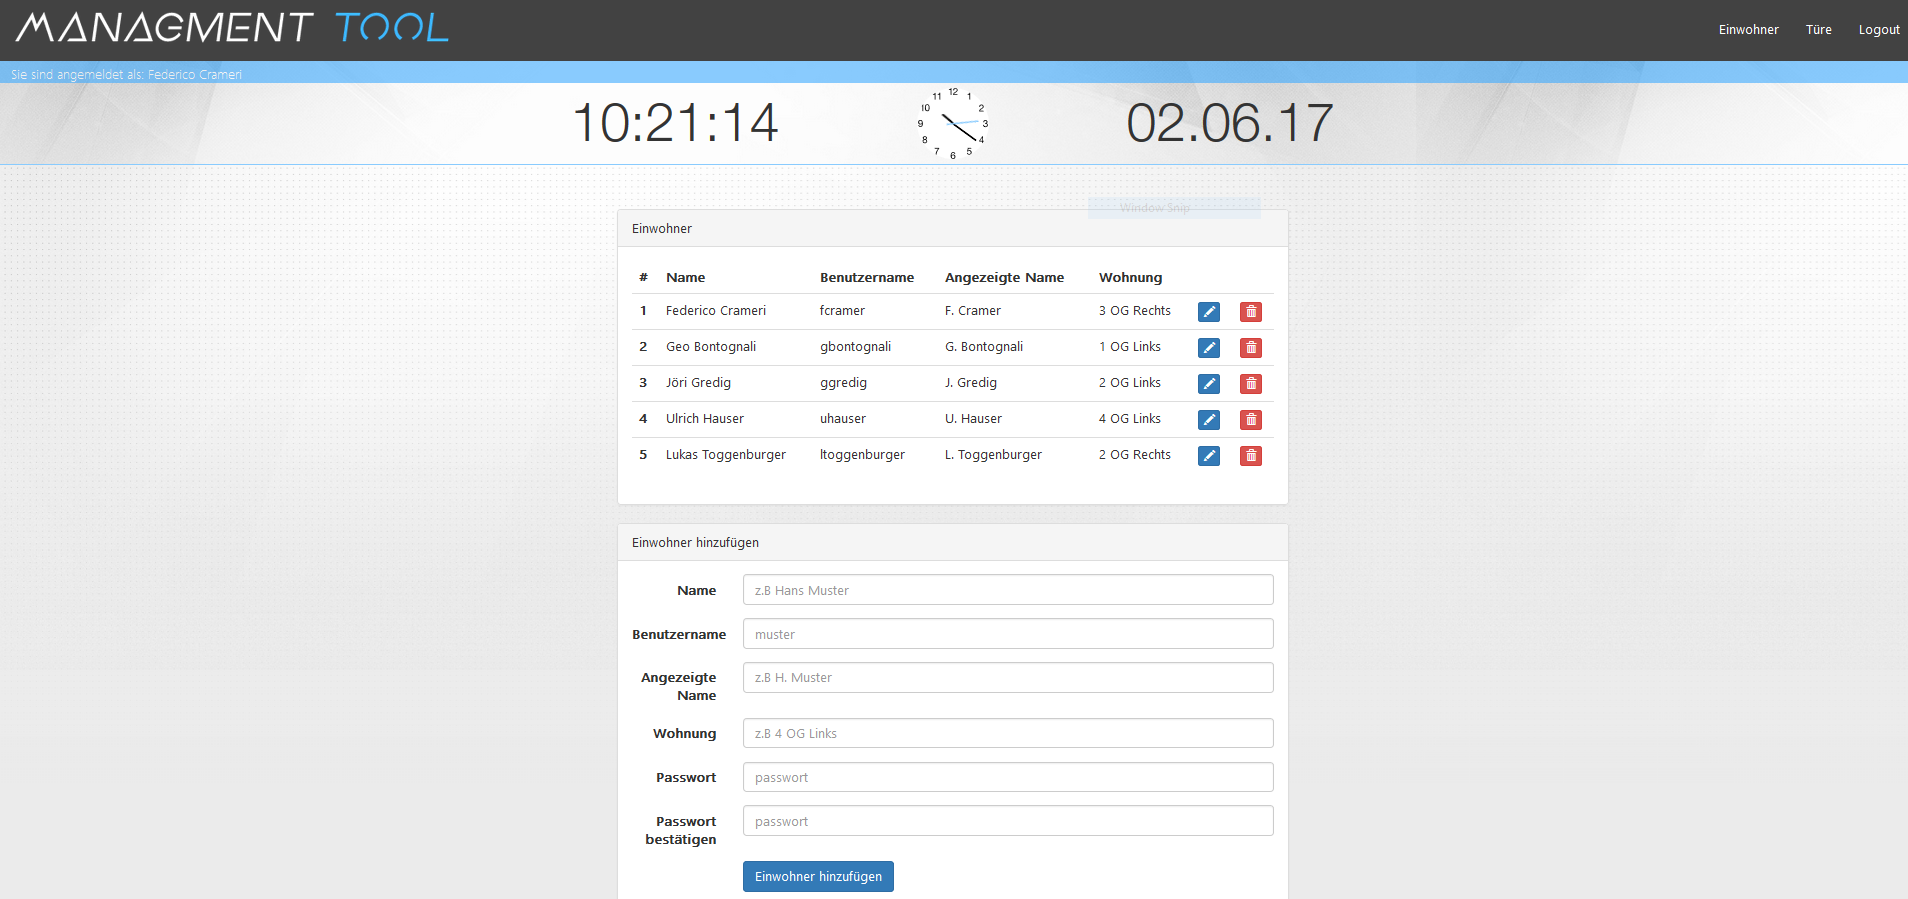
\includegraphics[width=1\textwidth]{managementtool}
		\caption[Design der Management tool]{Design der Management tool}
		\label{fig:managementtool}
	\end{center}
\end{figure}

Das Tool ist mit einem Login versehen und die Vertraulichkeit ist somit garantiert.
\\
\newline
\textbf{Bewohner} 
\\
Unter der Bewohnerseite werden alle Wohnungen, beziehungsweise alle Bewohner, aufgelistet. Diese verfügen über einen Benutzernamen und ein Passwort, die von der \gls{clientapp} verwendet werden um eine sichere Authentifizierung beim Server zu gewährleisten. In diesem Bereich hat man die Möglichkeit sowohl der Name als auch die Position der Wohnung, welche an der \gls{aussensprechstelle} angezeigt werden, abzuändern.
\\
\\
\textbf{Türen} 
\\
In diesem Abschnitt sind die Namen der Türen definiert, welche dann auf der \gls{clientapp} angezeigt werden. Der Einbau einer neuen Türe muss im \gls{managementtool} definiert werden. Dabei ist zu beachten, dass der ID mit demjenigen der auf der neu installierten \gls{aussensprechstelle} übereinstimmt. 
\\

\subsubsection{Remote Verbindung}
\label{kap:remote}
..


\subsection{OS und Dienste}
\label{kap:dienste}
Folgend beschrieben wir alle Dienste die auf dem Raspberry laufen werden. Diese werden benötigt um die Webapplikationen mit der Hardware zu verbinden.

\subsubsection{Raspbian}
\label{kap:raspbian}
Auf allen Raspberry Pi wurde der Betriebssystem Raspbian-Jessie installiert. Dieser wird von der Raspberry-Pi-Foundation mitgeliefert und gilt als besonders hochoptimierte \gls{os} für die mit niedriger Leistung und geringem Stromverbrauch \gls{arm} Prozessoren.
\\
 Raspbian basiert auf Debian welche unter der DFSG (Debian Free Software Guidelines) Lizenz steht. Diese erlaubt der unbeschränkten Weitergabe der Software sowie abgeleitete und modifizierte Werke weiterzugeben. Raspbian enthält Java SE Plattformprodukte welche unter dem BCL(Oracle Binary Code License) lizensiert sind. Diese Lizenz gewährleistet die obengenannten Freiheiten ebenfalls.
 \\

\subsubsection{Taster Controller}
Die \gls{aussensprechstelle} wird durch 3 Schalter bedient. Die Aufgabe der Taster-Controller besteht darin, die \gls{gpio}s der Raspberry, welcher mit den Schaltern verbunden sind, abzuhören. Sobald ein Schalter gedrückt wird, wird eine Tastatureingabe simuliert. Durch die Simulation kann der Javascript-Code, der lokal im Browser ausgeführt wird, auf den Schalterdruck reagieren. Somit kann auf der \gls{aussensprechstelle}, dank der Webapplikation (\seeref{fig:doordesign}), einen Bewohner ausgewählt werden (Schalter Rechts und Links) und diesen dann auch angerufen werden (Schalter Mitte).
\\
Ursprünglich wollten wir den Taster Controller, sowie alle anderen Dienste, als Daemon ausführen. Das hätte den Vorteil gehabt, dass der Daemon mittels eines üblichen Run-, Stop- oder Restart-Befehls gesteuert werden konnten. Per Definition ist ein Daemon benutzerunabhängig und genau dieser Ansatz war problematisch. Eine der eingesetzten Java-Library (Robot, um Keyevent zu simulieren) benötigt den Zugriff auf die \gls{lxde}-Desktopumgebung. Aus dem Grund, dass \gls{lxde} ein benutzerspezifischer Prozess ist, konnte der Taster-Controller nicht als Daemon ausgeführt werden.
\\
Um das Problem umzugehen bietet \gls{lxde} einen Autostart. Im Unix Runlevel 5 wird gewartet bis die Desktopumgebung initialisiert ist und der Taster-Controller wird erst dann ausgeführt. Somit kann jetzt die eingesetzte Robot-Library auf den \gls{lxde} zugreifen und die Tastatureingabe simulieren.
\\

\subsubsection{Speaker Controller}
Der Speaker-Controller ist ein kleiner Dienst, welcher den Lautsprecher ein- und ausschalten kann. Trotz einem Massentrennfilter sind immer noch leise Störsignale auf dem Audio-Ausgang vorhanden. Die Aufgabe des Speaker-Controllers besteht darin, die Stromspeisung des Speakers zu trennen, wenn er nicht verwendet wird. Somit ist das System energieeffizienter und unnötige Geräusche können vermieden werden. Der Speaker-Controller wird auf der \gls{aussensprechstelle} als Daemon ausgeführt.
\\
\\
Der Dienst besteht lediglich aus einem Socket-Server, der auf einem Signal wartet und durch die \gls{gpio} der Raspberry ein kleines Relais steuert. Das Signal kommt von der Javascriptseite der \gls{aussensprechstelle}-Webapplikation \textit{(localhost)} und kann so bei Bedarf den Lautsprecher ein- bzw. ausschalten.
\\

\subsubsection{Relay Controller}
Der Relais-Controller ist sehr ähnlich aufgebaut wie der Speaker-Controller. Auch hier handelt sich um einen kleinen Socket-Server, der auf ein Signal wartet und durch die GPIO des Raspberrys ein oder mehrere Relais steuert.
\\
Der Relais-Controller wird auf dem Server ausgeführt und wartet auf die Befehle der Webapplikationen. Das Relais ist am Türöffner und an den Gongs der Wohnungen angeschlossen.
\\
Der Datenaustausch zwischen dem Relais-Controller und den Webapplikationen erfolgt in Form eines \gls{json}-Strings.
\\
Während beim Speaker-Controller die Befehle aus der Clientseite stammen, kommen die Daten beim Relais-Controller aus dem \gls{json}-Backend vom Server selbst. Somit bleibt der Datenverkehr auf dem Localhost und werden Man-in-the-Middle oder Injection-Attacke ausgeschlossen. Aus diesem Grund lauscht dieser Server nur auf Verbindungen die vom Localhost stammen.

\subsection{Logging}
\label{kap:logs}
Für die Identifikation und Rückverfolgung von Fehlern sowie für den Monitoring sind Logs File von grosse Bedeutung. Diese werden bei allen Services und Dienste konsequent druchgeführt. Das Logrotate wird nicht eingesetzt, statdessen kümmert sich das Java runtime environment um die Grösse des generiertes Log Files. Aus dem Grund dass es sich noch um ein Protoyp handelt wurde das Logging Stufe auf 7 eingestellt. In diese Stufe werden alle Emergency Nachrichten bis auf die Debug Nachrichten im Log Dateien gespeichert.
Gemäss der FHS (Filesystem Hierarchy Standard) werden die Logs unter /var/log/Aussensprechstelle gesichert. 

Für die Identifikation und Rückverfolgung von Fehlern sowie für das Monitoring sind Logs-File von grosser Bedeutung. Diese werden bei allen Services und Dienste konsequent durchgeführt. 
\\
Das Logrotate wird nicht eingesetzt, stattdessen kümmert sich das Java-Runtime-Environment um die Grösse des generiertes Log-Files.  Da es sich noch um einen Prototyp handelt, wurde die Loggingstufe auf 7 eingestellt. Auf dieser Stufe werden alle Emergencynachrichten bis auf die Debugnachrichten in Logddateien gespeichert. 
\\
Gemäss dem FHS (Filesystem Hierarchy Standard) werden die Logs unter /var/log/Aussensprechstelle gesichert.

\subsection{Watchdog}
\label{kap:watchdog}
Die ganze Hardware, die an der Türe installiert wird, ist beim Endkunden schwer zugänglich. Sollte nun ein Problem mit dem System auftreten, müsste man die Anlage vor Ort zurücksetzen. In solchen Fällen hilft der Hardware-Watchdog, der auf dem Raspberry komplett unabhängig vom eigentlichen System läuft. 
\\
Der Vorteil eines Hardware-Watchdogs ist, dass wenn das System bzw. der Prozessor blockiert, diese unabhängige Hardware ihre Aufgabe weiterhin ausführt. Der Watchdog wird als standalone Gerät im Unix erkannt. Wird dieses Gerät einmal beschrieben, dann muss diese mit einem Zeitintervall von 15 Sekunden erneut beschrieben werden.
\\
Ist diese Bedingung nicht erfüllt, wird dann einen Hardware-Reset von Watchdog durchgeführt und das System wird neugestartet. Das Beschreiben vom Watchdog-Gerät wird von einer Watchdog-Daemon übernommen. Durch die Konfigurationsdatei des Daemons können verschiedene Parameter des Systems wie Temperatur, Auslastung der Prozessor usw. überwacht werden. Besonders relevant für die Türsprechanlage ist das PID-Monitoring. Diese ermöglicht das ständige Überprüfen von spezifischen Prozessen und Diensten die das System benötigt, um seinen Zweck als \gls{aussensprechstelle} zu erfüllen. 
\\
Sobald einer dieser Prozesse anhält wird das System innerhalb von 15 Sekunden neugestaltet. Ein solches Mechanismus steigert die Verfügbarkeit des Dienstes und ist für eine Türsprechanlage von grosser Bedeutung.


\newpage